\begin{frame}{Econ 57a, Environmental Economics, Fall 2019}
\protect\hypertarget{econ-57a-environmental-economics-fall-2019}{}

\begin{block}{Module 4: How to correct market failures}

\begin{itemize}
\tightlist
\item
  Pigouvian tax
\item
  Coase theorem, cap-and-trade
\item
  Weitzman, Price vs.~Quantity
\item
  Ostrom and institutional solutions
\end{itemize}

\end{block}

\end{frame}

\begin{frame}{}
\protect\hypertarget{section}{}

In this module, we are going to talk about:

\begin{itemize}
\tightlist
\item
  Should the government intervene?
\item
  If so, how?
\item
  If not, what are the alternatives?
\end{itemize}

\end{frame}

\begin{frame}{}
\protect\hypertarget{section-1}{}

Governmental interventions are often necessary when free markets cannot
achieve efficient outcomes:

\begin{itemize}
\tightlist
\item
  Anti-trust laws to correct monopoly
\item
  Lemon laws, disclosure of vehicle history to correct for assymetric
  information
\item
  Environmental regulations to correct externality from pollution
\end{itemize}

In fact, some of the most important functions for the government are 1)
providing public goods 2) establish and protect property right and
market institutions; and 3) correcting market failures

\end{frame}

\begin{frame}{Different types of intervention}
\protect\hypertarget{different-types-of-intervention}{}

\begin{itemize}
\tightlist
\item
  Prescriptive Regulation
\item
  Market-based Approach
\item
  Information-based Approach
\end{itemize}

\end{frame}

\begin{frame}{}
\protect\hypertarget{section-2}{}

So, how should the government intervene to ``internalize'' the
externalities?

\end{frame}

\begin{frame}{The mining pollution example (from the last module)}
\protect\hypertarget{the-mining-pollution-example-from-the-last-module}{}

Red Keep LLC can mine the uranium with a marginal private cost (MPC) of:
\textbf{P = Q}. It also generates an marginal external cost (MEC) of
\textbf{\$10} per unit. The marginal social cost is thus \textbf{P = Q +
10}.

The market demand for uranium is: \textbf{P = 30 - Q}

\end{frame}

\begin{frame}{}
\protect\hypertarget{section-3}{}

A socially efficient equilibrium is: \(Q^* = 10\), and \(P^* = 20\)

Private market will arrive at: \(Q' = 15\), and \(P' = 15\)

\end{frame}

\begin{frame}{}
\protect\hypertarget{section-4}{}

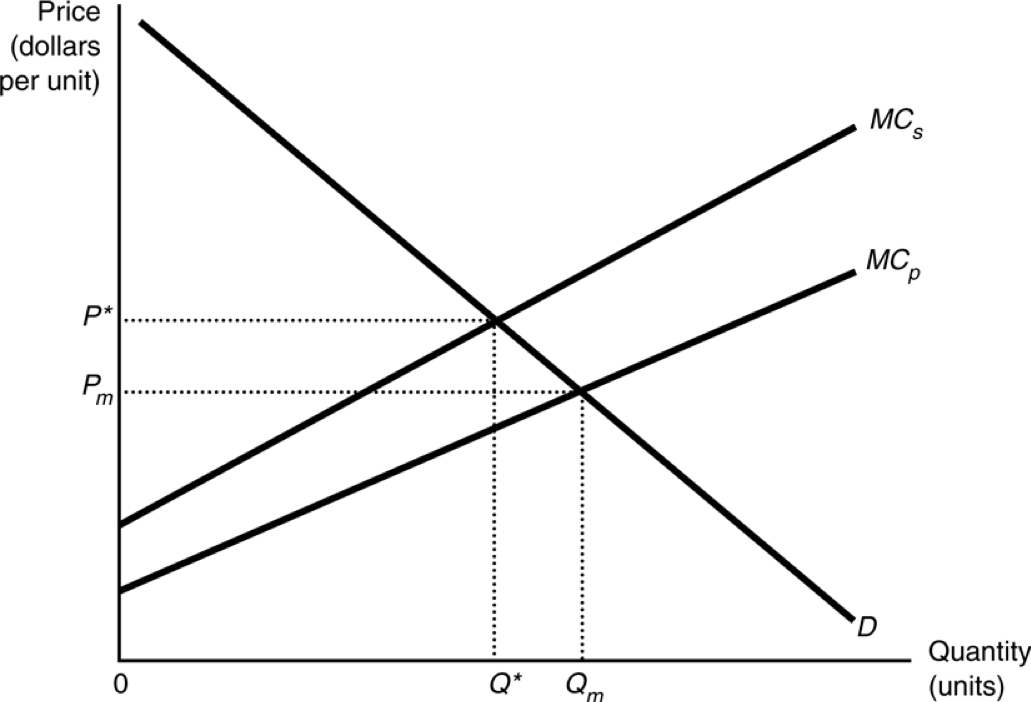
\includegraphics[width=\textwidth,height=4.16667in]{figures/m3_marginal_social_cost.png}

\end{frame}

\begin{frame}{}
\protect\hypertarget{section-5}{}

\begin{itemize}
\tightlist
\item
  There exists an externality (pollution) that is not internalized in
  the market
\item
  The marginal private cost is lower than the marginal social cost
\item
  Firms overshoots production, sells at a lower price comparing to the
  efficient outcome
\end{itemize}

\end{frame}

\begin{frame}{The tax instrument}
\protect\hypertarget{the-tax-instrument}{}

One particular way to do so is to put a \textbf{pollution tax} on the
firm. The tax is often referred to as the \textbf{Pigovian tax}, named
after A.C. Pigou, an English economist, in the 1920s.

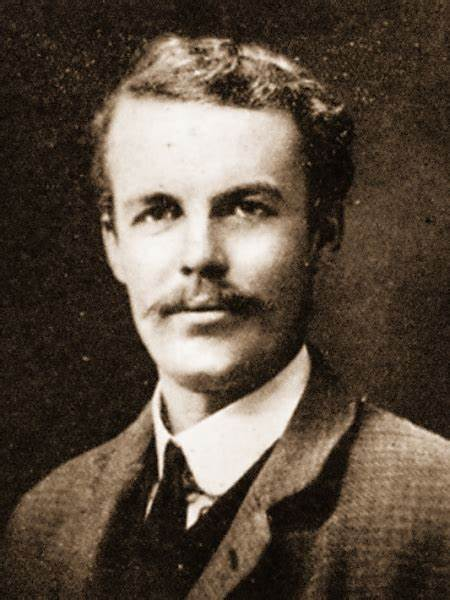
\includegraphics[width=\textwidth,height=3.125in]{figures/m4_pigou.jpeg}

\end{frame}

\begin{frame}{}
\protect\hypertarget{section-6}{}

The idea is simple:

\begin{itemize}
\tightlist
\item
  Set the tax rate equals to the marginal external cost at the
  equilibrium
\item
  The polluter has to pay the tax in addition to production costs, thus
  lower their production
\item
  Market failure is corrected through internalizing the external cost of
  pollution
\end{itemize}

\end{frame}

\begin{frame}{Tax instrument in the mining example}
\protect\hypertarget{tax-instrument-in-the-mining-example}{}

The producer faces a MPC of \textbf{P = Q}, plus a pollution tax of
\textbf{t=10}. Thus the actual cost for the producer becomes

\textbf{P = Q + 10}

Equating the supply with the demand of \textbf{P = 30 - Q}, we get:

\(Q^* = 10\), and \(P^* = 20\)

which is exactly the socially optimal price and quantity.

\end{frame}

\begin{frame}{}
\protect\hypertarget{section-7}{}

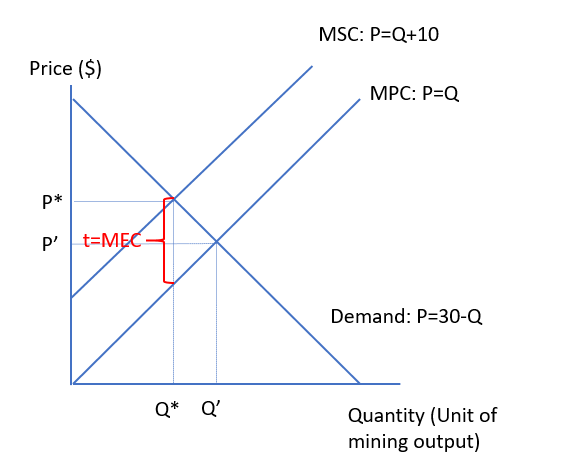
\includegraphics[width=\textwidth,height=4.6875in]{figures/m4_mining_tax.png}

\end{frame}

\begin{frame}{Real world examples of (proposed) pollution taxes:}
\protect\hypertarget{real-world-examples-of-proposed-pollution-taxes}{}

\begin{itemize}
\tightlist
\item
  Gasoline tax
\item
  Carbon tax
\item
  Wastewater discharge levies
\end{itemize}

\end{frame}

\begin{frame}{}
\protect\hypertarget{section-8}{}

Pigouvian policies are in theory efficient, but not without caveats:

\begin{itemize}
\tightlist
\item
  Sound economic policy may not be politically popular
\item
  Tax is a ``bad'' word, especially in this country
\item
  Especially problematic if the tax involves a personal choice: are we a
  ``nanny state'' or what?
\item
  Hard to adjust the tax rate once it becomes law, even if new
  information pours in
\end{itemize}

\end{frame}

\begin{frame}{}
\protect\hypertarget{section-9}{}

Wait a minute. Is there another way?

\end{frame}

\begin{frame}{}
\protect\hypertarget{section-10}{}

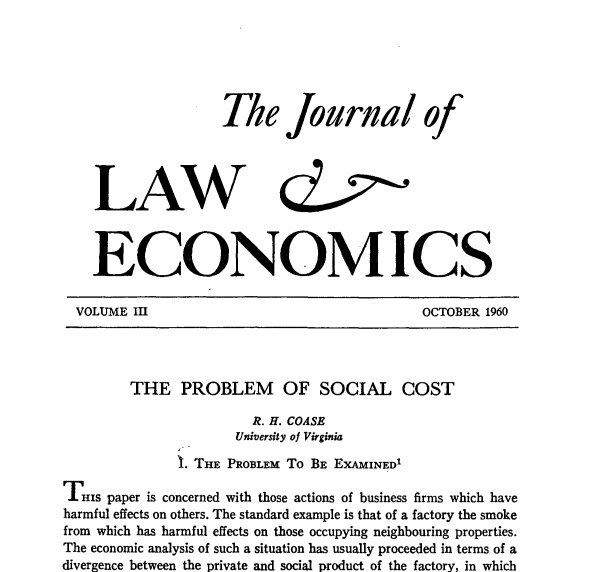
\includegraphics[width=\textwidth,height=4.6875in]{figures/m4_the_problem_of_social_cost.png}

\end{frame}

\begin{frame}{}
\protect\hypertarget{section-11}{}

The idea is simple: assign the property right to either party, and let
them negotiate with each other.

\begin{itemize}
\tightlist
\item
  If residents have the right to enjoy clean water supply, then the
  mining company will pay the residents in order to pollute
\item
  If the mining company has the right to pollute, then residents will
  pay the company for it NOT to pollute
\end{itemize}

\end{frame}

\begin{frame}{The Coase theorem}
\protect\hypertarget{the-coase-theorem}{}

\textbf{If property rights are well-defined, and there are no
transaction costs, then no matter what the initial allocation of
resources, negotiation between parties will reach a pareto-optimal
outcome WITHOUT interventions from the government.}

\end{frame}

\begin{frame}{How is the Coase theorem useful?}
\protect\hypertarget{how-is-the-coase-theorem-useful}{}

All we need is a ``clearly-defined'' property right structure, and then
we can:

\begin{itemize}
\tightlist
\item
  Let the court decide who has the right to the good
\item
  Let the parties trade with each other: cap-and-trade
\item
  Privatize the good at large
\end{itemize}

\end{frame}

\begin{frame}{TQs from you}
\protect\hypertarget{tqs-from-you}{}

I strongly identify myself with the notions of the Coase Theorem. I
believe that when you get to the grassroots level of human welfare,
individuals looking to have the best outlooks for other is the
foundation of a just society \ldots{} The elimination of government in
matters of environmental economics leaves the solution to be dealt with
the parties involved where the two, three or however many don't lose any
benefit from unnecessary government intervention.

President Reagan ran on the notion the government isn't the solution to
problems but itself is the problem. A hands off approach by government
would give the proper room for those involved to settle the
environmental issue.

\end{frame}

\begin{frame}{The Mock Trial}
\protect\hypertarget{the-mock-trial}{}

Jon Snow vs.~Daenerys Targaryen (2019)

\end{frame}

\begin{frame}{Paper I gave Jon}
\protect\hypertarget{paper-i-gave-jon}{}

Your name is Lord Jon Snow, a rancher living near the Long Lake, a small
lake in the state of Wyoming. The lake is the only freshwater source
nearby, and your herd of cattle depends on that lake to survive.
Unfortunately, a farmer nearby named Daenerys Targaryen also wants
control for the Long Lake to irrigate her field, and there is no way
that the lake can be shared between you two. You think you are entitled
to the right to use the lake, so you decide to take her to court.

According to the best of your estimate, the lake generates \$X worth of
value to you. That is, if you lose control of the lake, there will be
about \$X worth of economic damage to your cattle.

\end{frame}

\begin{frame}{Paper I gave Dany}
\protect\hypertarget{paper-i-gave-dany}{}

Your name is Queen Daenerys Targaryen, a farmer/landowner living near
the Long Lake, a small lake in the state of Wyoming. The lake is the
only freshwater source nearby, and your farmland depends on that lake to
remain irrigated. Unfortunately, a rancher nearby named Jon Snow also
wants control for the Long Lake to feed his cattle, and there is no way
that the lake can be shared between you two. You think you are entitled
to the right to use the lake, so you decide to take him to court.

According to the best of your estimate, the lake generates \$Y worth of
value to you. That is, if you lose control of the lake, there will be
about \$Y worth of economic damage to your cattle.

\end{frame}

\begin{frame}{The polluter-pays principle}
\protect\hypertarget{the-polluter-pays-principle}{}

Assigning the ``right to clean environment'' to the public: polluters
have to seek permission from the public (pay) in order to pollute.

\begin{itemize}
\tightlist
\item
  Usually a point-source affects a broader community

  \begin{itemize}
  \tightlist
  \item
    coordination problem\\
  \end{itemize}
\item
  Avoids moral hazard

  \begin{itemize}
  \tightlist
  \item
    If smokers have the right to smoke, they will just extort
    non-smokers
  \end{itemize}
\item
  Discourages entry into polluting industry
\end{itemize}

\end{frame}

\begin{frame}{Basic Components of a Cap-and-Trade are:}
\protect\hypertarget{basic-components-of-a-cap-and-trade-are}{}

\begin{enumerate}
\tightlist
\item
  Establish a policy cap, i.e., the optimal quantity of pollution
  emission/resource extraction for the society
\item
  Issue permits to the polluters/extractors with the total amount of
  quota equal to the cap
\item
  Each polluter's emission cannot exceed the amount of quota they hold
\item
  Establish a market for the polluters to trade their quotas with each
  other
\end{enumerate}

\end{frame}

\begin{frame}{What changed?}
\protect\hypertarget{what-changed}{}

\begin{enumerate}
\tightlist
\item
  The permit (and the pollution at large) is now a private good:
\end{enumerate}

\begin{itemize}
\tightlist
\item
  Exclusivity: Only the firm holding the permit can emit
\item
  Rivalry: One firm ``consuming'' the permit reduces the amount that
  other firms can emit
\item
  Transferability: the permit can be transfered in a marketplace
\end{itemize}

\begin{enumerate}
\setcounter{enumi}{1}
\tightlist
\item
  There is now a market to trade these permits:
\end{enumerate}

\begin{itemize}
\tightlist
\item
  Externality exists because ``markets do not reflect the true benefit
  or cost of one's action''
\item
  Market price is the best signal to indicate the scarcity of a resource
\end{itemize}

\end{frame}

\begin{frame}{Quantity instrument in the fishery example}
\protect\hypertarget{quantity-instrument-in-the-fishery-example}{}

Recall the fishery problem last time, where an open-access resource
faces rent dissipation:

\begin{itemize}
\tightlist
\item
  After a certain point, new entry to the fishery decreases everybody
  else's catch
\item
  An open-access fishery will be overfished because the fishery cannot
  limit entry
\end{itemize}

\end{frame}

\begin{frame}{}
\protect\hypertarget{section-12}{}

\begin{itemize}
\tightlist
\item
  Marginal benefit for the fishery given numbers of boats B is
  \textbf{100 - 4B}
\end{itemize}

\[MC = 10\]

\end{frame}

\begin{frame}{}
\protect\hypertarget{section-13}{}

For the fishery to have the highest positive benefit, we need to solve:

\textbf{Marginal Benefit = Marginal Cost}

where MB is the slope of the total benefit, or \[10 = 100 - 4B\]
\[B^*=22.5\]

\end{frame}

\begin{frame}{An open-access outcome is characterized by:}
\protect\hypertarget{an-open-access-outcome-is-characterized-by}{}

\textbf{Total Benefit = Total Cost}

where at such point each and every boat just breaks even from the
fishery. Notice that the total cost is just \textbf{TC=10B}, we have:

\[100B - 2B^2 = 10B\]

\[B^{OA}=45\]

\end{frame}

\begin{frame}{Alaska's Salmon Regulation}
\protect\hypertarget{alaskas-salmon-regulation}{}

\begin{itemize}
\tightlist
\item
  In the 1950s, Pacific salmon fisheries were over-exploited
\item
  Government decided to act:

  \begin{itemize}
  \tightlist
  \item
    Shorten fishing periods
  \item
    Restrict fishing technology

    \begin{itemize}
    \tightlist
    \item
      Prohibit the use of nets/traps
    \item
      Banned engine-powered fishing boats!
    \end{itemize}
  \end{itemize}
\end{itemize}

\end{frame}

\begin{frame}{}
\protect\hypertarget{section-14}{}

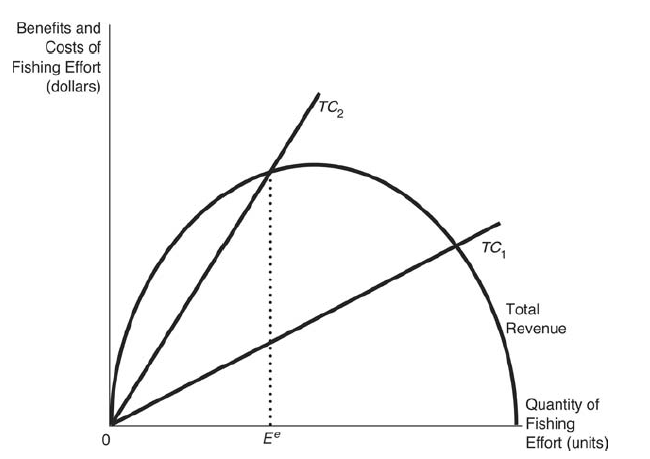
\includegraphics[width=\textwidth,height=4.6875in]{figures/m4_fishing_limit_effort.png}

\end{frame}

\begin{frame}{Rights-based policies}
\protect\hypertarget{rights-based-policies}{}

Give 22.5 units of permits to all fisherman/woman, i.e., limits B*=22.5

\end{frame}

\begin{frame}{}
\protect\hypertarget{section-15}{}

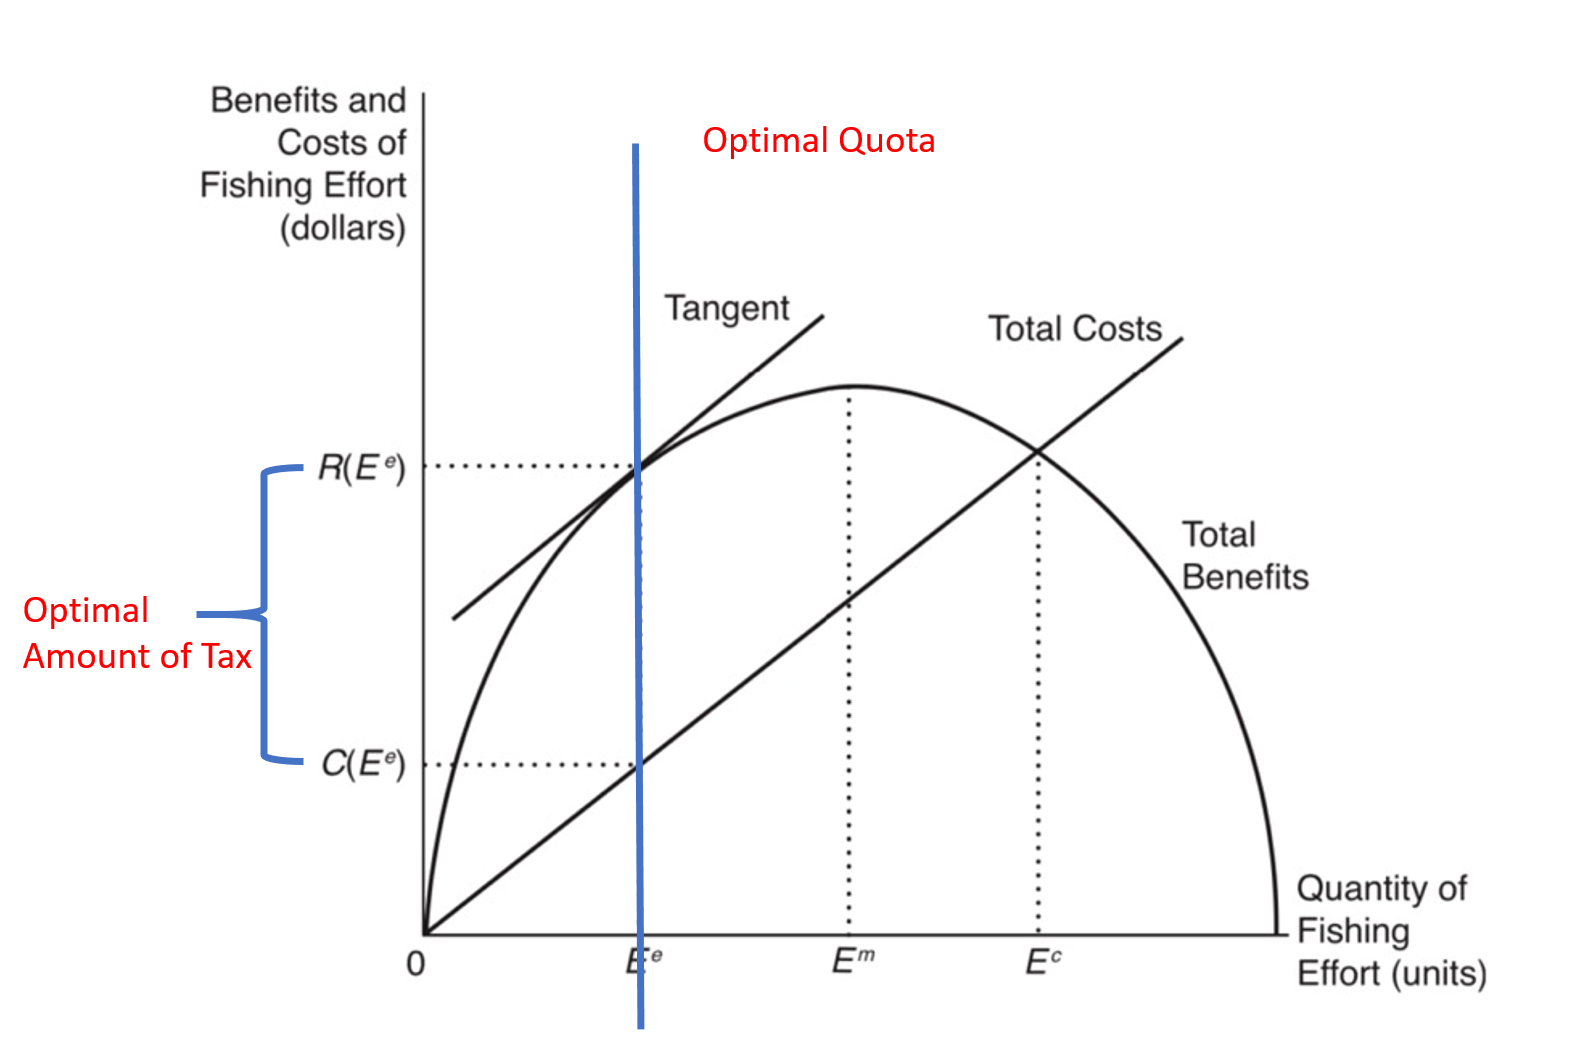
\includegraphics[width=\textwidth,height=4.6875in]{figures/m4_fishery_instrument.png}

\end{frame}

\begin{frame}{}
\protect\hypertarget{section-16}{}

Rights-based approach works better:

\begin{itemize}
\tightlist
\item
  Individual Veseel Quota (IVQ)

  \begin{itemize}
  \tightlist
  \item
    Only works in the short-run
  \end{itemize}
\item
  Invidiaul Fishing Quota (IFQ)
\item
  Individual Transferable Quota (ITQ)
\item
  Territorial Use Rights Fisheries (TURF)
\end{itemize}

\end{frame}

\begin{frame}{}
\protect\hypertarget{section-17}{}

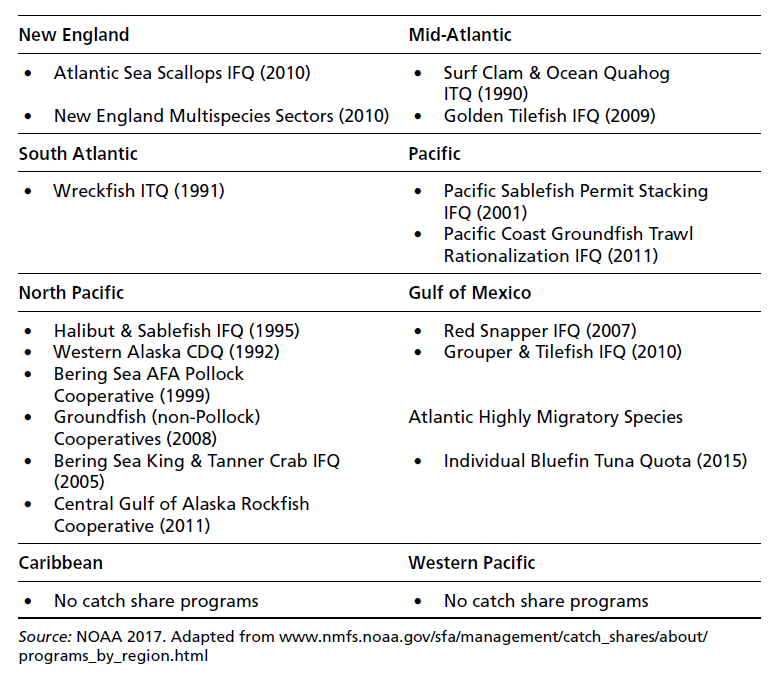
\includegraphics[width=\textwidth,height=4.6875in]{figures/m4_fishing_regulation.png}

\end{frame}

\begin{frame}{Alaska's ITQ restriction (Kroetz 2017)}
\protect\hypertarget{alaskas-itq-restriction-kroetz-2017}{}

Permits (quota) assigned to vessel sizes:

\begin{itemize}
\tightlist
\item
  A(Unrestricted size and type), B(35-60ft), and C(\textless35ft)
\item
  Quotas are traded within each vessel category
\end{itemize}

What's gonna happen?

\end{frame}

\begin{frame}{Real-world rights-based programs}
\protect\hypertarget{real-world-rights-based-programs}{}

\begin{itemize}
\tightlist
\item
  Wetland Banking
\item
  Air pollution Cap-and-trade (sulfur, carbon, mercury, nitrogen)
\item
  Fishing quotas
\end{itemize}

\end{frame}

\begin{frame}{Caveats about Cap-and-Trade}
\protect\hypertarget{caveats-about-cap-and-trade}{}

\begin{itemize}
\tightlist
\item
  Prices are volatile

  \begin{itemize}
  \tightlist
  \item
    Affected by 1) policy shocks 2) market shocks
  \end{itemize}
\item
  Needs strong governmental backup

  \begin{itemize}
  \tightlist
  \item
    Solidity of the property rights
  \end{itemize}
\item
  Create pollution hot spots

  \begin{itemize}
  \tightlist
  \item
    Trading partners may not necessarily locate within proximity
  \item
    Environmental justice concerns
  \end{itemize}
\end{itemize}

\end{frame}

\begin{frame}{}
\protect\hypertarget{section-18}{}

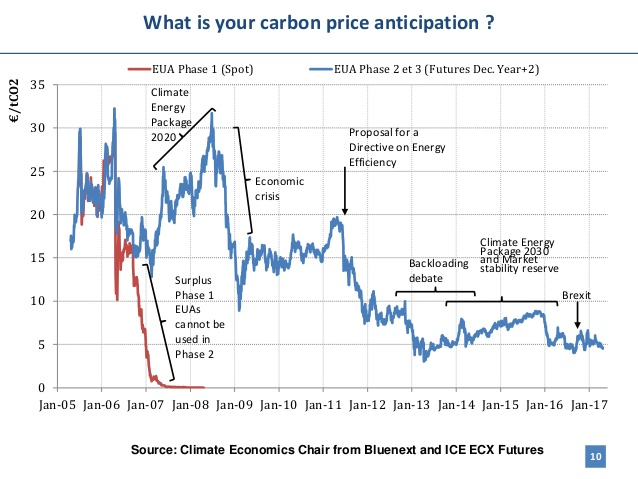
\includegraphics[width=\textwidth,height=4.6875in]{figures/m4_euets_prices.jpg}

\end{frame}

\begin{frame}{}
\protect\hypertarget{section-19}{}

If tax and cap-and-trade are equivalent, then what is the fuss about
choosing carbon tax or carbon trading?

\end{frame}

\begin{frame}{}
\protect\hypertarget{section-20}{}

\begin{itemize}
\item
  Congressman O'Rourke: Cap-and-Trade
\item
  then Congressman Markey: the 2009 bill
\item
  Andrew Yang: Carbon Tax at \$40/ton
\item
  Mayor Buttigieg: Carbon Tax
\item
  Senator Booker: Carbon fee
\end{itemize}

\end{frame}

\begin{frame}{}
\protect\hypertarget{section-21}{}

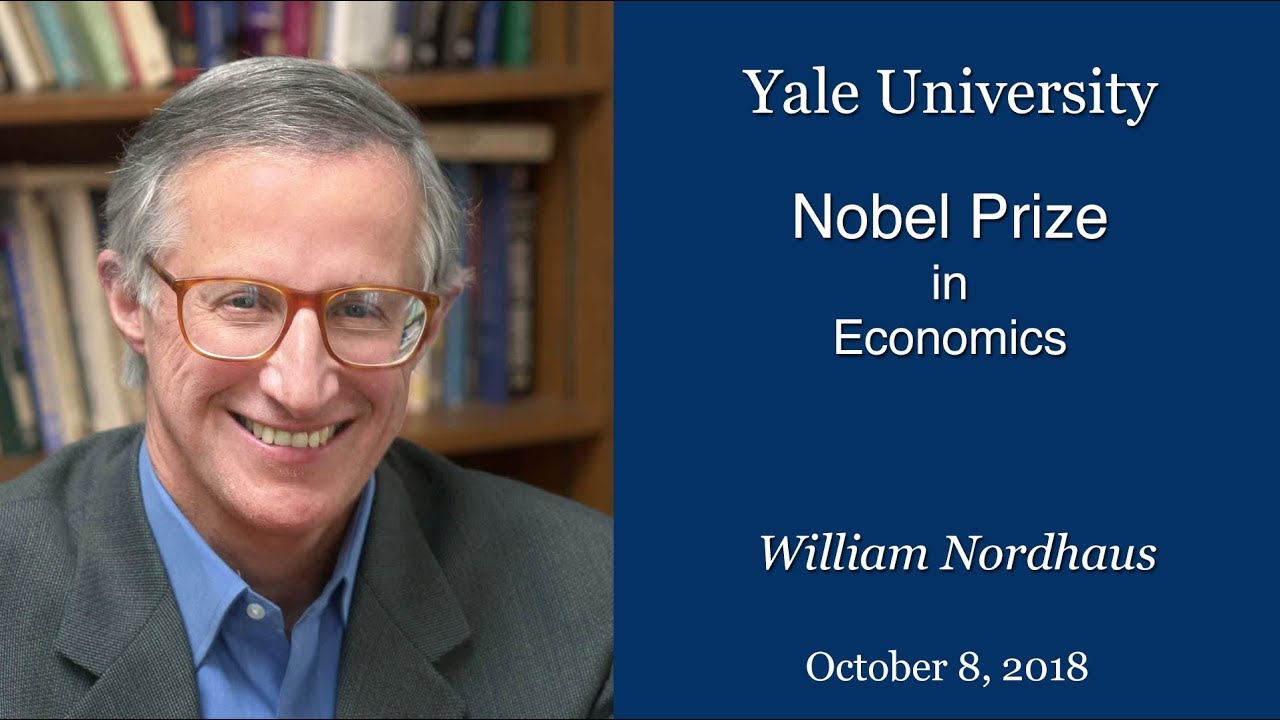
\includegraphics[width=\textwidth,height=2.60417in]{figures/m4_nordhaus.jpg}


\includegraphics[width=\textwidth,height=2.60417in]{figures/m4_weitzman.png}

\end{frame}

\begin{frame}{}
\protect\hypertarget{section-22}{}

\begin{itemize}
\tightlist
\item
  Nordhaus: Structural modeling on the ``Social Cost of Carbon''

  \begin{itemize}
  \tightlist
  \item
    A ``know-it-all'' model
  \item
    Advocates for carbon tax
  \end{itemize}
\item
  Weitzman: what really matters is the tail events, not the average

  \begin{itemize}
  \tightlist
  \item
    Prevent catastrophic events
  \item
    Advocates for cap-and-trade
  \end{itemize}
\end{itemize}

\end{frame}

\begin{frame}{The Role of Uncertainty}
\protect\hypertarget{the-role-of-uncertainty}{}

\begin{itemize}
\tightlist
\item
  If the regulator has complete information about marginal costs, then
  tax and cap-and-trade are equivalent
\item
  Not necessarily the case

  \begin{itemize}
  \tightlist
  \item
    Uncertainty in measurement
  \item
    Innovation
  \item
    Firms reporting strategically
  \end{itemize}
\end{itemize}

\end{frame}

\begin{frame}{Prices vs.~Quantities}
\protect\hypertarget{prices-vs.-quantities}{}

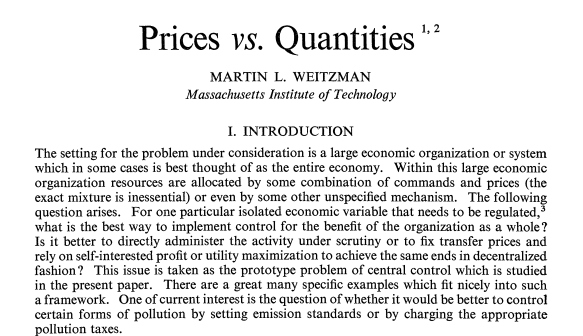
\includegraphics[width=\textwidth,height=4.6875in]{figures/m4_weitzman1974.png}

\end{frame}

\begin{frame}{}
\protect\hypertarget{section-23}{}

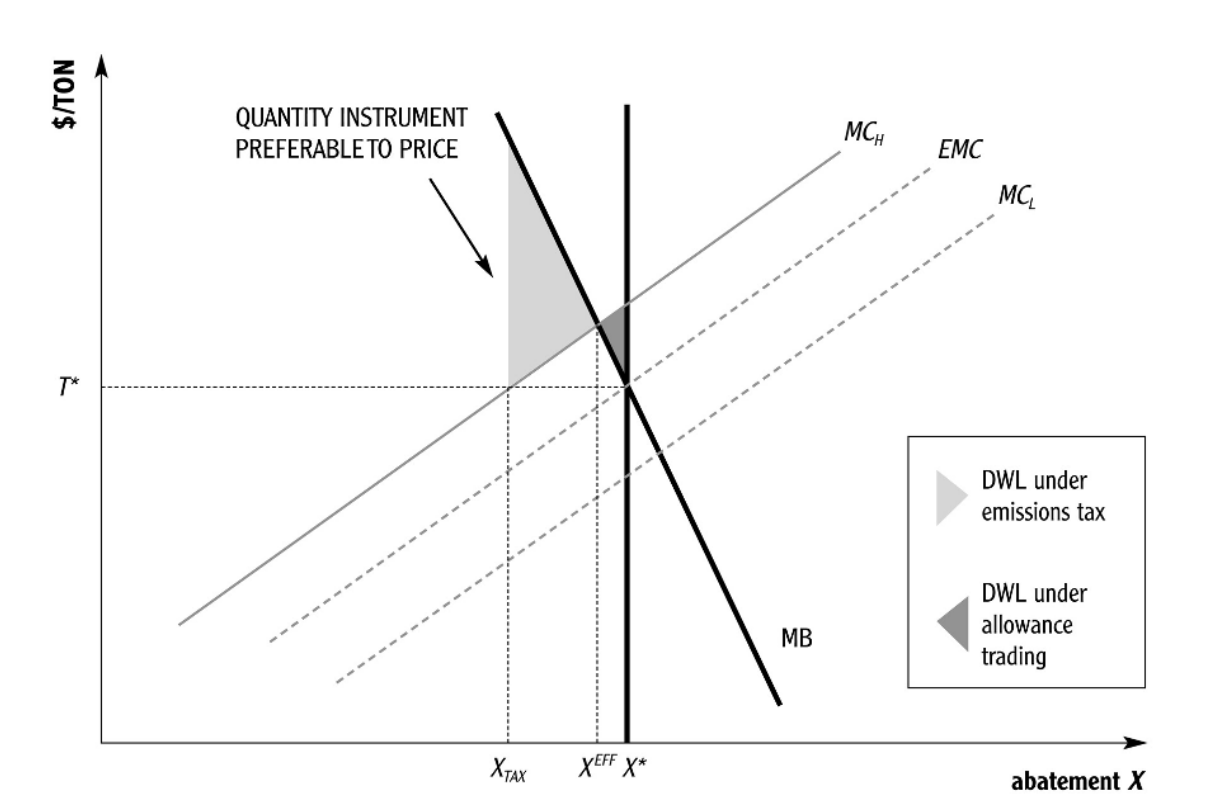
\includegraphics[width=\textwidth,height=4.6875in]{figures/m4_pvq1.png}

\end{frame}

\begin{frame}{}
\protect\hypertarget{section-24}{}

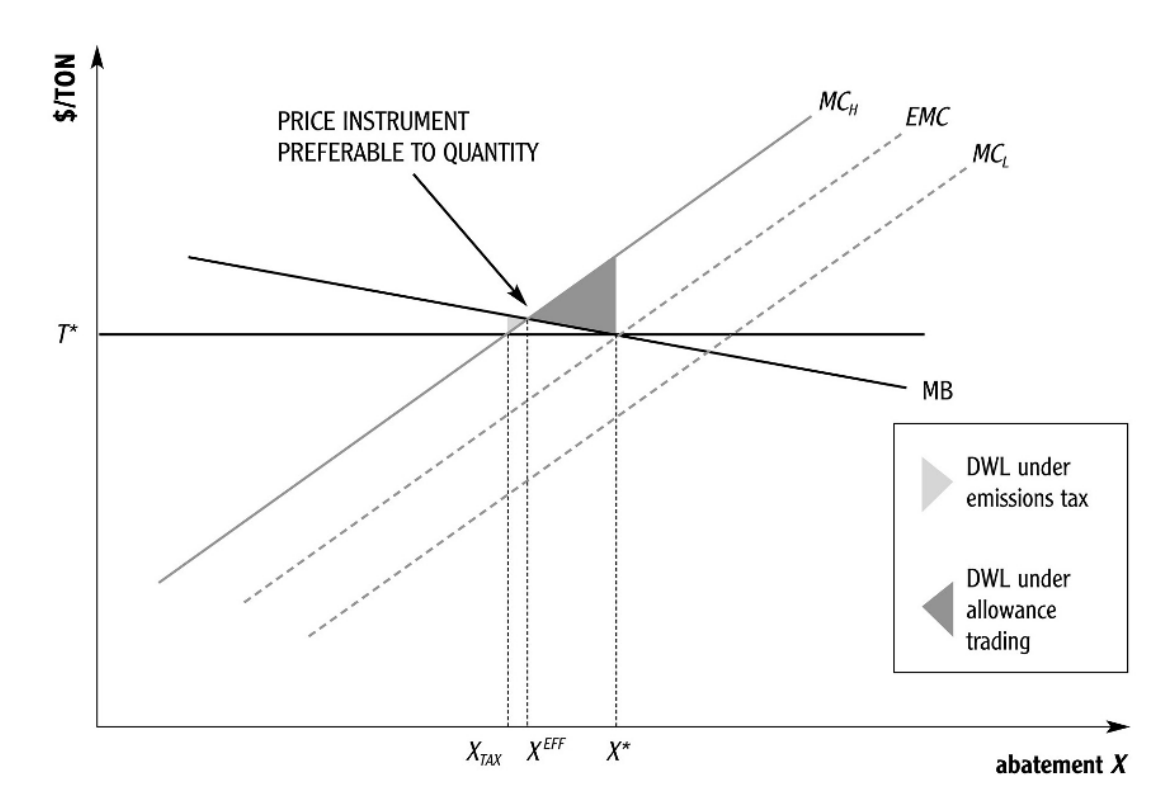
\includegraphics[width=\textwidth,height=4.6875in]{figures/m4_pvq2.png}

\end{frame}

\begin{frame}{}
\protect\hypertarget{section-25}{}

\begin{itemize}
\tightlist
\item
  Tax is preferred when MC is steeper than MB

  \begin{itemize}
  \tightlist
  \item
    Getting the price right is more important
  \end{itemize}
\item
  Cap-and-trade is preferred when MB is steeper than MC

  \begin{itemize}
  \tightlist
  \item
    Getting the quantity right is more important
  \end{itemize}
\end{itemize}

\end{frame}

\begin{frame}{Are common-pool resources always better governed by
governmental regulation?}
\protect\hypertarget{are-common-pool-resources-always-better-governed-by-governmental-regulation}{}

\end{frame}

\begin{frame}{The Case for Privatization (Enclosure)}
\protect\hypertarget{the-case-for-privatization-enclosure}{}

Coase theorem also clearly suggests that if property rights are
clearly-defined, then the resource allocation will be efficient.

\end{frame}

\begin{frame}{Trophy Hunting}
\protect\hypertarget{trophy-hunting}{}

\begin{itemize}
\tightlist
\item
  Poaching is a huge threat to African wildlife
\item
  Especially elephants, but also Buffalo, Antelope, etc.
\end{itemize}

\end{frame}

\begin{frame}{}
\protect\hypertarget{section-26}{}

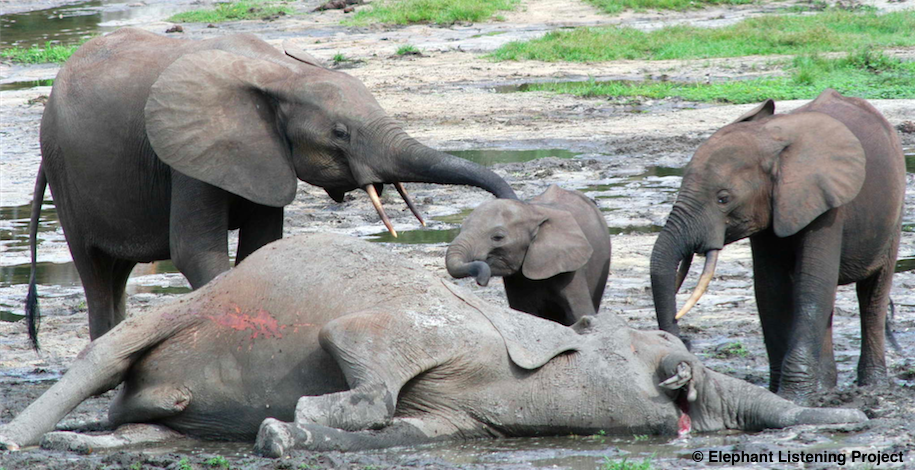
\includegraphics[width=\textwidth,height=4.6875in]{figures/m4_elephant.png}

\end{frame}

\begin{frame}{}
\protect\hypertarget{section-27}{}

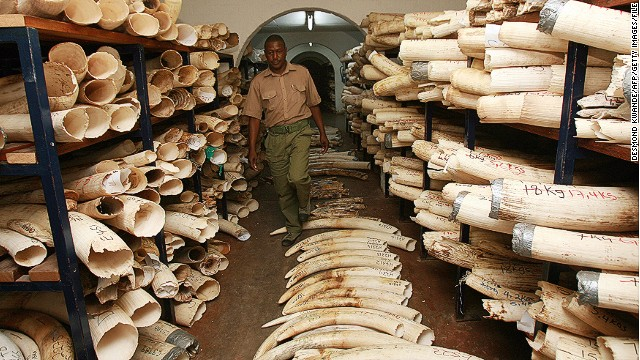
\includegraphics[width=\textwidth,height=4.6875in]{figures/m4_ivory.jpg}

\end{frame}

\begin{frame}{}
\protect\hypertarget{section-28}{}

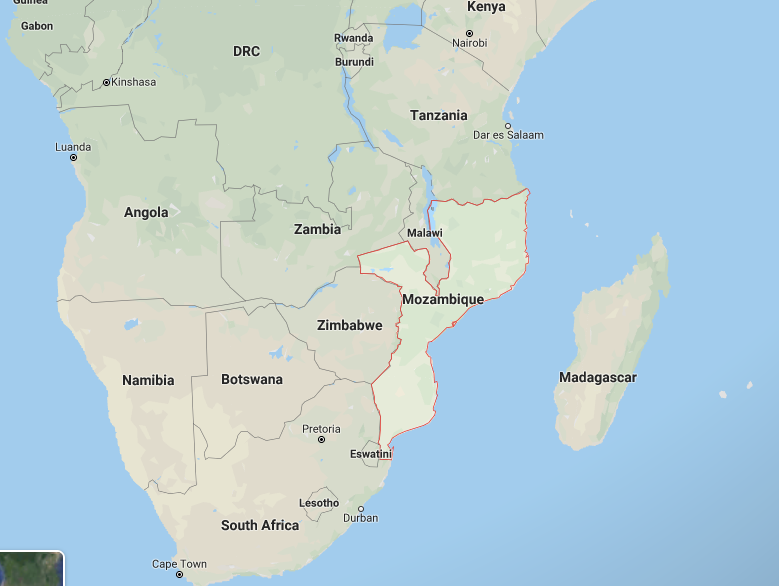
\includegraphics[width=\textwidth,height=4.6875in]{figures/m4_mozambique.png}

\end{frame}

\begin{frame}{A bit about Mozambique}
\protect\hypertarget{a-bit-about-mozambique}{}

\begin{itemize}
\tightlist
\item
  Per capita GDP of \$415
\item
  Independence war 1964-1975, Civil War 1977-1992
\end{itemize}

\end{frame}

\begin{frame}{Coutada 11: the Meat Locker}
\protect\hypertarget{coutada-11-the-meat-locker}{}

\begin{itemize}
\tightlist
\item
  Coutada: ``Hunting District'', one district is roughly the size of the
  Grand Canyon National Park
\item
  Warring factions go there to shoot bush meat to feed rebels and
  national army
\item
  Russians go in with helicoptor gunships to hunt Cape Buffalo, can
  them, and ship them to Afghanistan
\item
  Locals ``poach'' to feed the family
\item
  By 1994, only 2100 Cape Buffalo and 44 Sable Antelope were left
\end{itemize}

\end{frame}

\begin{frame}{}
\protect\hypertarget{section-29}{}

In year 1994, a South African named Mark Haldane leased Coutada 11 from
the Mozambique government

\begin{itemize}
\tightlist
\item
  Mark is a hunter himself
\item
  Has business in Zimbabwe and South Africa
\end{itemize}

\end{frame}

\begin{frame}{}
\protect\hypertarget{section-30}{}

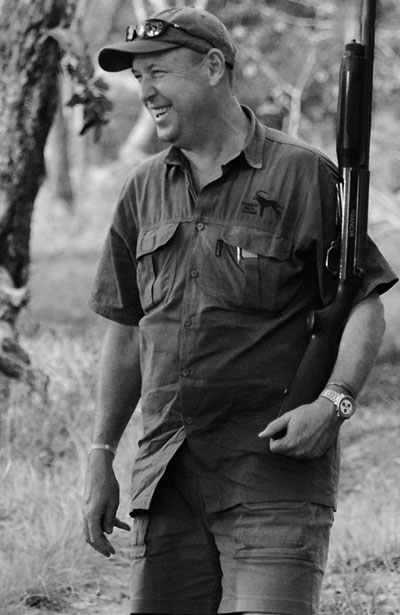
\includegraphics[width=\textwidth,height=4.6875in]{figures/m4_haldane.jpg}

\end{frame}

\begin{frame}{}
\protect\hypertarget{section-31}{}

Mark wanted to set up a trophy hunting program in the area to attract
wealthy Westerners, so he worked with the locals:

\begin{itemize}
\tightlist
\item
  Give back the meat to the local villages

  \begin{itemize}
  \tightlist
  \item
    Most locals can't afford an adequate diet
  \end{itemize}
\item
  Give the locals job opportunities

  \begin{itemize}
  \tightlist
  \item
    Hired 150 people in the camp
  \item
    20-plus men anti-poaching patrol, most used to poach themselves
  \item
    Make sure outsiders do not come in and poach
  \end{itemize}
\end{itemize}

\end{frame}

\begin{frame}{}
\protect\hypertarget{section-32}{}

Trophy hunting site opens up:

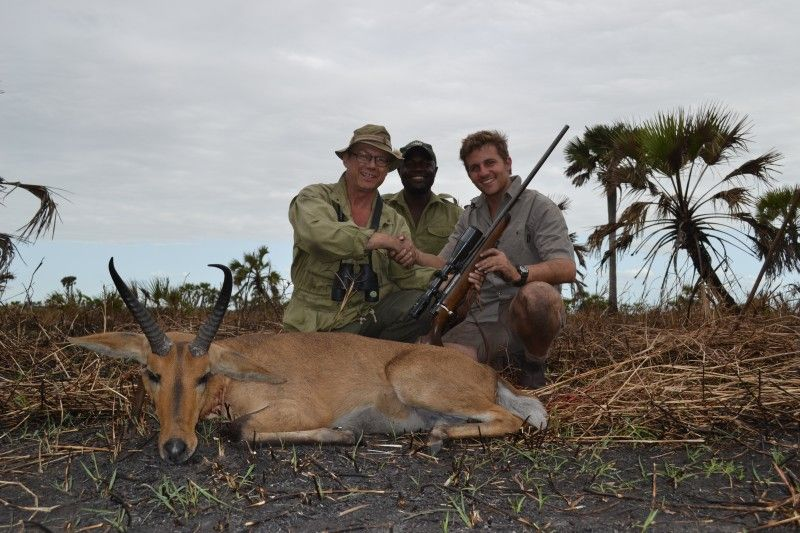
\includegraphics[width=\textwidth,height=4.16667in]{figures/m4_trophy_hunting.jpg}

\end{frame}

\begin{frame}{What happened after a couple of years?}
\protect\hypertarget{what-happened-after-a-couple-of-years}{}

Cape Buffalo: from 2100 to over 21000 Sable Antelope: from 44 to over
5000

And, financially, the program is completely self-sustainable.

\end{frame}

\begin{frame}{}
\protect\hypertarget{section-33}{}

Question: why is that?

\end{frame}

\begin{frame}{}
\protect\hypertarget{section-34}{}

\begin{itemize}
\tightlist
\item
  Turning an open-access resource into a private resource:

  \begin{itemize}
  \tightlist
  \item
    Exclusivity
  \item
    Enforceability
  \end{itemize}
\item
  Provide incentives to the locals
\end{itemize}

\end{frame}

\begin{frame}{}
\protect\hypertarget{section-35}{}

Any problems/concerns with the approach?

\end{frame}

\begin{frame}{}
\protect\hypertarget{section-36}{}

\begin{itemize}
\tightlist
\item
  Animal welfare?
\item
  Other non-hunting values?
\end{itemize}

\end{frame}

\begin{frame}{}
\protect\hypertarget{section-37}{}

\begin{quote}
Most modern economic theory describes a world presided over by a
government (not, significantly, by governments), and sees this world
through the government's eyes. The government is supposed to have the
responsibility, the will and the power to restructure society in
whatever way maximizes social welfare; like the US Cavalry in a good
Western, the government stands ready to rush to the rescue whenever the
market `fails', and the economist's job is to advise it on when and how
to do so. Private individuals, in contrast, are credited with little or
no ability to solve collective problems among themselves. This makes for
a distorted view of some important economic and political issues.
-Sugden(1986)
\end{quote}

\end{frame}

\begin{frame}{Coase and Pigou represent two alternate school of
thoughts}
\protect\hypertarget{coase-and-pigou-represent-two-alternate-school-of-thoughts}{}

\begin{itemize}
\tightlist
\item
  Government as the Leviathan

  \begin{itemize}
  \tightlist
  \item
    Command and Control, Tax, or Issuing Permits
  \item
    Market failure has to be corrected by governmental intervention
  \end{itemize}
\item
  Privatization as the Magic Wand

  \begin{itemize}
  \tightlist
  \item
    Clearly define property rights of the common-pool resources
  \end{itemize}
\item
  Tragedy of the commons cannot be avoided if these prescriptions are
  not adopted.
\end{itemize}

\end{frame}

\begin{frame}{This is far from reality}
\protect\hypertarget{this-is-far-from-reality}{}

\begin{itemize}
\tightlist
\item
  Self-regulated irrigation systems in Nepal, Spain, Phillipines

  \begin{itemize}
  \tightlist
  \item
    Irrigation systems usually suffer from the collective action problem
  \item
    Self-regulated via informal talks amongst farmers
  \item
    More efficient \& effective than government-managed rules
  \end{itemize}
\end{itemize}

\end{frame}

\begin{frame}{}
\protect\hypertarget{section-38}{}

\begin{itemize}
\tightlist
\item
  Fishing in the Cree Nation of Hudson Bay, Canada

  \begin{itemize}
  \tightlist
  \item
    Long-lasting social rules that govern how to fish
  \item
    Violators face social disgrace as well as mild penalty
  \end{itemize}
\item
  Other fisheries in Turkey, Sri Lanka
\end{itemize}

\end{frame}

\begin{frame}{Top-down approach may not work well in reality in those
situations}
\protect\hypertarget{top-down-approach-may-not-work-well-in-reality-in-those-situations}{}

The top-down approach will need:

\begin{itemize}
\tightlist
\item
  Knowledge about localized benefit and costs
\item
  Strong, local enforcement
\item
  Free of corruption
\end{itemize}

\end{frame}

\begin{frame}{}
\protect\hypertarget{section-39}{}

Recall that in the one-shot prisoner's dilemma game, self-interested
individuals end up in a socially non-optimal (Nash) equilibrium.

What if the game is not played ``one-shot'', but are played for multiple
rounds?

\end{frame}

\begin{frame}{Axelrod's Tournament}
\protect\hypertarget{axelrods-tournament}{}

In 1980, Robert Axelrod, professor of political science at the
University of Michigan, held a tournament of various strategies for the
prisoner's dilemma.

The basic rule of the tournament is this:

\begin{itemize}
\tightlist
\item
  Each player is paired with another random player in the pool
\item
  The game is going to play 200 rounds
\item
  The final score is the sum of total scores in all rounds
\end{itemize}

\end{frame}

\begin{frame}{Different strategies emerge}
\protect\hypertarget{different-strategies-emerge}{}

\begin{itemize}
\tightlist
\item
  ``The Fool'': One who always corporates
\item
  ``The Cheat'': One who always defects
\item
  ``The Unpredictable'': One who randomly chooses to corporates or
  defects
\end{itemize}

\end{frame}

\begin{frame}{}
\protect\hypertarget{section-40}{}

\begin{itemize}
\tightlist
\item
  The Tit for Tat: cooperates on the first move, and mimic what the
  other play did on the previous move

  \begin{itemize}
  \tightlist
  \item
    retaliates if the other player defects
  \end{itemize}
\item
  The Tit for Two Tat:

  \begin{itemize}
  \tightlist
  \item
    retaliates if the other play defects two times in a roll
  \end{itemize}
\item
  The Two Tit for Tat

  \begin{itemize}
  \tightlist
  \item
    retaliates two times if the other play defects
  \end{itemize}
\end{itemize}

\end{frame}

\begin{frame}{}
\protect\hypertarget{section-41}{}

\begin{itemize}
\tightlist
\item
  ``The Grudger'':

  \begin{itemize}
  \tightlist
  \item
    Cooperate until the other play defect, then defect forever
  \end{itemize}
\item
  ``The Opportunist'':

  \begin{itemize}
  \tightlist
  \item
    start with tic-for-tat, but randomly defects every 5-15 moves,
    hoping others won't find out
  \end{itemize}
\item
  ``The Gradual Punisher''

  \begin{itemize}
  \tightlist
  \item
    retaliates one time for the first defect, two times for the second,
    \ldots{}
  \end{itemize}
\end{itemize}

\end{frame}

\begin{frame}{}
\protect\hypertarget{section-42}{}

The ``Tideman and Chieruzzi''

\begin{enumerate}
\item
  Every run of defections played by the opponent increases the number of
  defections that this strategy retaliates with by 1.
\item
  The opponent is given a `fresh start' if:
\end{enumerate}

\begin{itemize}
\tightlist
\item
  it is 10 points behind this strategy
\item
  and it has not just started a run of defections
\item
  and it has been at least 20 rounds since the last `fresh start'
\item
  and there are more than 10 rounds remaining in the match
\item
  and the total number of defections differs from a 50-50 random sample
  by at least 3.0 standard deviations.
\end{itemize}

\end{frame}

\begin{frame}{Who wins?}
\protect\hypertarget{who-wins}{}

Benchmark:

\begin{itemize}
\tightlist
\item
  Defect while the other cooperate: 1000
\item
  All cooperate: 600
\item
  All defect: 200
\item
  Cooperate while the other defect: 0
\end{itemize}

\end{frame}

\begin{frame}{}
\protect\hypertarget{section-43}{}

With a maximum of 600 points, here they are:

\begin{itemize}
\tightlist
\item
  Tit-for-tat: 504
\item
  Tideman and Chieruzzi: 500
\item
  The Gradual Punisher: 480.7
\item
  The Grudger: 473
\item
  The Opportunist: 400
\item
  The Random: 276
\end{itemize}

\end{frame}

\begin{frame}{The Follow up Tournaments}
\protect\hypertarget{the-follow-up-tournaments}{}

\begin{itemize}
\tightlist
\item
  The second tournament:

  \begin{itemize}
  \tightlist
  \item
    62 submissions, full knowledge of others in the pool ahead of time
  \item
    Tit-for-tat comes in first
  \end{itemize}
\item
  The evolutionary tournament:

  \begin{itemize}
  \tightlist
  \item
    Number of strategies in the pool ties to how well that strategy did
    in the previous round
  \item
    Survival for the fittest
  \item
    Tic-for-tat wins again
  \end{itemize}
\end{itemize}

\end{frame}

\begin{frame}{Implications from Axelrod's Tournament}
\protect\hypertarget{implications-from-axelrods-tournament}{}

\begin{itemize}
\tightlist
\item
  The prisoner's dilemma is not necessarily a dilemma in the long-run
\item
  Be a ``nice guy'' is evoluntionarily compatible
\item
  Punishment is necessary
\end{itemize}

\end{frame}

\begin{frame}{How does that help governing the commons}
\protect\hypertarget{how-does-that-help-governing-the-commons}{}

\begin{itemize}
\tightlist
\item
  Cooperation is achievable without governmental intervention or
  privatization of the resource
\item
  Trust can be gained through ``reciprocity'': good will exchanges
  between individuals
\item
  Still face the risk of ``defection''
\end{itemize}

\end{frame}

\begin{frame}{Ostrom's Observation}
\protect\hypertarget{ostroms-observation}{}

Rather than using a pen and a pencil, Ostrom really went into the field:

\begin{itemize}
\tightlist
\item
  Study a large number of institutions that work empirically
\item
  Detailed information about those institutions
\item
  Document common features, look for regularities
\item
  Needs more sophisticated, qualitative theory
\end{itemize}

\end{frame}

\begin{frame}{What does she find?}
\protect\hypertarget{what-does-she-find}{}

Ostrom's principles of designing long-surviving institutions

\begin{enumerate}
\tightlist
\item
  Define boundaries clearly
\item
  Design FAIR rules to use the resource (usually proportional to the
  benefit)
\item
  Involve the participants into the rule-making process
\item
  Monitor and enforce these rules locally
\item
  Apply gradual sanctions to violators
\end{enumerate}

\end{frame}

\begin{frame}{The power of norms}
\protect\hypertarget{the-power-of-norms}{}

These principles are usually conveyed through norms

\begin{itemize}
\tightlist
\item
  Humans are evolutionarily adapted to follow norms
\item
  Norms are monitored by the entire community
\item
  Passed along generation-by-generation (repeated games)
\end{itemize}

\end{frame}

\begin{frame}{}
\protect\hypertarget{section-44}{}

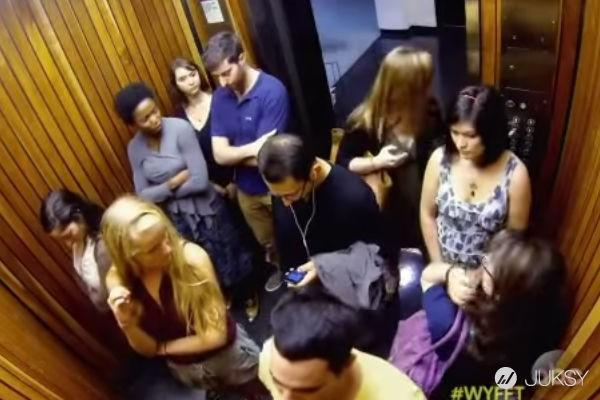
\includegraphics[width=\textwidth,height=4.16667in]{figures/m4_elevator.jpg}

\end{frame}

\begin{frame}{What can threaten these self-governing rules?}
\protect\hypertarget{what-can-threaten-these-self-governing-rules}{}

\end{frame}

\begin{frame}{}
\protect\hypertarget{section-45}{}

\begin{itemize}
\tightlist
\item
  Outside forces (national government, international aids) trying to
  impose a uniformed standard
\item
  Rapid change in technology/monetary input
\item
  Transmission failure when passing along to the next generation
\item
  Corruption
\item
  Lack of fair and low-cost conflict resolution mechanisms
\end{itemize}

\end{frame}

\begin{frame}{Takeaways from this module}
\protect\hypertarget{takeaways-from-this-module}{}

There are three schools of thought to correct market failure:

\begin{itemize}
\tightlist
\item
  Taxation (Pigou)
\item
  Clarify property rights (Coase)

  \begin{itemize}
  \tightlist
  \item
    Create market for public/common-pool goods
  \item
    Privatization
  \item
    Litigation
  \end{itemize}
\item
  Cooperative institutions

  \begin{itemize}
  \tightlist
  \item
    Potentially works, but are fragile
  \end{itemize}
\end{itemize}

\end{frame}
